\documentclass {life-en}
\usepackage{eurosans}
\usepackage{totpages}

\begin{document}

\title{La Vie Est Un Jeu}
\subtitle{Specifications}
\member{Lepage Barbara}{lepage.barbara@gmail.com}
\member{Caradec Guillaume}{guillaume.caradec@gmail.com}
\member{Corsin Simon}{simoncorsin@gmail.com}
\member{Glorieux Francois}{fra.glorieux@gmail.com}
\member{Klarman Nicolas}{nickoas@gmail.com}
\member{Lassagne David}{david.lassagne@gmail.com}
\member{Louvigny Guillaume}{guillaume@louvigny.fr}
\member{El-Outmani Youssef}{youssef.eloutmani@gmail.com}
\member{Le-Cor Wilfried}{wilfried.lecor@gmail.com}
\member{Lenormand Frank}{lenormf@gmail.com}

\summary
{
        The purpose of the specification is to set the requirements for making our service.
}

\maketitle
\authorspageen

%% ------------------------------------------------ % ---------------------%

\chapter*{Summary}
{
  ``La Vie Est Un Jeu'' is a 3-year project as part of ``Epitech
  Innovative Projects'' with a group of 10 students.\\
  \\
  This project, as a website and mobile applications, offers
  users to excite their day. To do this, they are offered a
  fun way to set goals, achieve them, collect them
  and then share them.\\
  It is therefore both a game and a social network, for all ages!\\
  \\
  The website will show as the first view some presentation slide of
  the project. The user's home page, once connected, will contain a
  short flow of information (eg when a user has set a
  objective) or a long one: when a user has made a goal and is sharing it.
  \\\\
  The user profile page will contain an array of medals representing
  the goals he has done. We call the achieved targets as
  ``Achievements'', in relation to those that can be found in games
  Videos\\
  \\
  The project will be using a new and innovating technology:
  Ocsigen, a powerful web server and framework in OCaml.\\
  The web server will be hosted on a Dedibox.\\
  \\
  The team will work wisely in order to complete the project
  despite the distance between the members. Indeed, throughout the second
  years of the project, members will be scattered across all
  the world for one academic year abroad required.\\
  \\
  This project is ambitious by its technical challenge, with the use of a
  little known technology, but also by its sought success from its future users.
}

\chapter*{Document Informations}

\begin{tabular}{| m{5cm} | m{10cm} |}
  \hline
  Document Type & Specifications \\
  \hline
  Group Name & ``La Vie Est Un Jeu'' \\
  \hline
  Number of pages & \ref{TotPages} \\
  \hline
  Full title of the document & Specifications Project ``La Vie Est Un Jeu'' \\
  \hline
  Authors & Members of the group, see cover page \\
  \hline
  Manager & Group Leader: Barbara Lepage \\
  \hline
  Contact & lavieestunjeu@googlegroups.com \\
  \hline
  Keywords & ``specifications'', ``lavieestunjeu'' \\
  \hline
  Current revision & 2.1 \\
  \hline
  Showcase website & http://eip.epitech.eu/2014/lavieestunjeu/ \\
  \hline
  Official Website & Not Available \\
  \hline
\end{tabular}

\chapter*{Table of revisions}

\revision{1.0}{Lepage Barbara}{Reminder EIP}{05/04/2012}
\revision{1.1}{Louvigny Guillaume}{Basic principle for the future system}{05/04/2012}
\revision{1.2}{Lepage Barbara}{Hardware environment}{05/04/2012}
\revision{1.3}{Lenormand Frank}{Environment realizable}{05/04/2012}
\revision{1.4}{Lenormand Frank}{Technical Architecture}{05/04/2012}
\revision{1.5}{Klarman Nicolas}{Security Management}{05/04/2012}
\revision{1.6}{Lepage Barbara}{Sensitive points}{05/04/2012}
\revision{1.7}{Le-Cor Wilfried}{Description of the tests first level}{05/04/2012}
\revision{1.8}{Lassagne David}{Diagram of the database}{05/04/2012}
\revision{2.0}{Lepage Barbara}{Updated Summary and redesign of global}{01/07/2012}
\revision{2.1}{Louvigny Guillaume}{Resumption of mobile applications and some minor corrections}{05/07/2012}
\revision{2.2}{Corsin Simon}{Corrected translations}{05/07/2012}

\listofrevisions

\newpage

\tableofcontents


%% ------------------------------------------------ % ---------------------%

\chapter{Introduction}

This specification is a contractual document to define the
specification of ``La Vie Est Un Jeu'', our EIP. \\
It specifies the set of features, in addition to site architecture and
mobile applications.\\
The internal structure of the database will also be described.\\
This document will also detail the potential targets of the project and try to 
estimate the financial and time constraints required to complete this project.\\
Finally, the opening provided to third party developers will also be discussed.


%% ------------------------------------------------ % ---------------------%

\chapter{Epitech, EIP and ``La Vie Est Un Jeu''}

\section{Epitech, a computer school like no other}

Epitech is a school computer experts. Its educational projects
directly involves students in their learning and makes them better able
to react and adapt easily, for example to technological developments which
will be held during their career.

\section{The EIP, a key component of academic success}

An Epitech Innovative Project or EIP is the key element of the Epitech's curriculum. This is a graduation project involving a minimum of six students around a common goal. This project is conducted over a period of three years, much larger than those of projects completed in the first three years of study. In addition, the EIP asks students to confront the enterprise world.

\section{``La Vie Est Un Jeu'', more than just EIP: a revolution!}

As part of our EIP, we decided to make a fun social network based on "lists of things to do before you die": it defines all the things the author wants to make during its existence, a kind of memo not to ruin his life. Our project will allow our visitors to build their own lists and validate their achievements while sharing them with their social networks. Thus, each action performed by a user (adding an activity, success or failure) will be a thread in which visitors and their networks can discuss and share different types of media on it(photos, videos, etc..). This thread will be on the own information flow of each one. The activity of a user is validated by its own network and will appear as a "success", as in a video game. The site will eventually offering other characteristics specific to video games.

%% ------------------------------------------------ % ---------------------%

\chapter{Requirements and project information}

\section{Recipients of the project}

Users targeted by the project are numerous. A person who has a hobbie or a passion covered by the site may have enough reason to sign up.\\

The site as mobile applications are designed for an extended internationalization.

\section{Using the project, compared to existing}

For end users, the project will consist of a website and several mobile applications including Android, iOS and Windows Phone. For third party developers, an API will be created allowing the creation of new uses.\\

The project is created to respond to a set of features not present in existing projects. These combined features are not present on the sites or competitors. Indeed, we wish to establish a platform playful enough to be visited daily, without neglecting the social aspect allowing visitors discussing their leisure in their network and sharing his experiences through photos and videos .\\

After the first year of project work in partnership with INRIA and KOALAB Epitech, we believe to have a functional site. During the second year of work on the EIP we would like to sign commercial partnerships with various actors in cultural areas or events. This period will also be an opportunity to add new features that meet new needs from users.

\newpage

\section{Re-technological context}

Today, more and more Internet users are equipped with smartphones, it is even provided that the number of Internet mobile users will exceeds the number of settled Internet users within a few years.\\
\\
To front this change and cope with the significant expansion of new technologies, we chose to offer to our users a fat client to each major mobile platforms.

\section{What is a ``Achievement''?}
The term achievement (which is like a success) is, in gaming, a goal set by the player, outside the main goal (which is win or finish the game).\\
The Achievements are awards which add challenge for the player.\\
\\
We could use a French translation of the term achievement but we believe that this one is most popular in the gaming world.\\
\\
The Achievements allow the player to explore more deeply the game content and therefore to explore new horizons.\\
The achievement is often a good time for the player.\\
He feels a certain satisfaction and feels rewarded for the effort.\\
It can then share with his friends to collect the honors or challenge their friends to do the same or better, which greatly improves the immersion in the game \\
\\
We believe, it is interesting to draw an analogy with life.\\
The life is a game like any other and also deserves its Achievements.

\section{Goal Final Project}

The project aims to create a user community around a system of "Achievements", directly related to everyday life, passions or professional life.\\

Targeted users are very numerous. In theory, anyone with a hobby or passion is a target.\\

In the longer term, business partnership will target specific brands and locations.\\

The site will be multilingual, so open to internationalization.

%% ------------------------------------------------ % ---------------------%

\chapter{Description of the different parts of the Internet and mobile services}

\section{The Website}

\subsecti on{Overview of the homepage before login}

The user will see first a slide show highlighting some "Achievements", arranged by date of publication and popularity, and the various functions of the site. This slide will aim to encourage the user to register.\\

The home page will also allow the user to register in the site. This registration is detailed below.\\

The last main feature of this home page is the ability for a user to login in the site.\\

The entrance could eventually help to find out the "Achievements" and its categories.

\newpage

\subsection{The inscription, the first five minutes!}

The objective of this step is clearly to avoid the heaviness caused by the information gathering the site needs to do with the future user (presenting a wild compact form is likely to scare him and making him to cancel his registration).\\

So we thought to a single-step mode system in which , while the user discovers our tool and its world, ask him subtle inquiries on a regular basis, in order to lighten this essential step which allow us to categorize the new registrant and offer contents based on these collected information.\\

In addition of combining the role of "guide" for the site discovery and "pollster" for information gathering, this method has the advantage of pushing the user to finish the presentation, and thus the registration. As the registration step continueas and when the group advanced (psychological effect, he wants to finish what he started, having already begun to contribute as well go all the way). The presentation from the growing interest, the chances increase of a registration upon arrival.\\
\\

In the present state we can imagine as a first approach a simple question that leads to a single action mode "you are one click to enter our universe" with, for example, the choice of gender: Male, Female, Not stated .

\begin{figure} [H]
  \begin{center}
    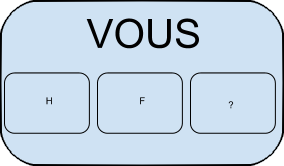
\includegraphics [width = 10cm]{img/vous.png}
  \end{center}
\end{figure}

\newpage

\subsection{The user home page once logged}

The home page of the user used the site presents its information flow, like the usual stream sites such as Facebook or Google +. \\

The menu must be discreet. The user should immediately see the four main tabs:

\begin{itemize}
  \item flow (default homepage);
  \item the user's objectives (the inscriptions);
  \item "Achievements";
  \item "friends" of the user (or imported ajoutables social networks within the site).
\end{itemize}

A bar of "breaking news" constantly on top of the site will give the user the latest in a line "Achievements" to his friends and the new homepage.

\begin{figure} [H]
  \begin{center}
    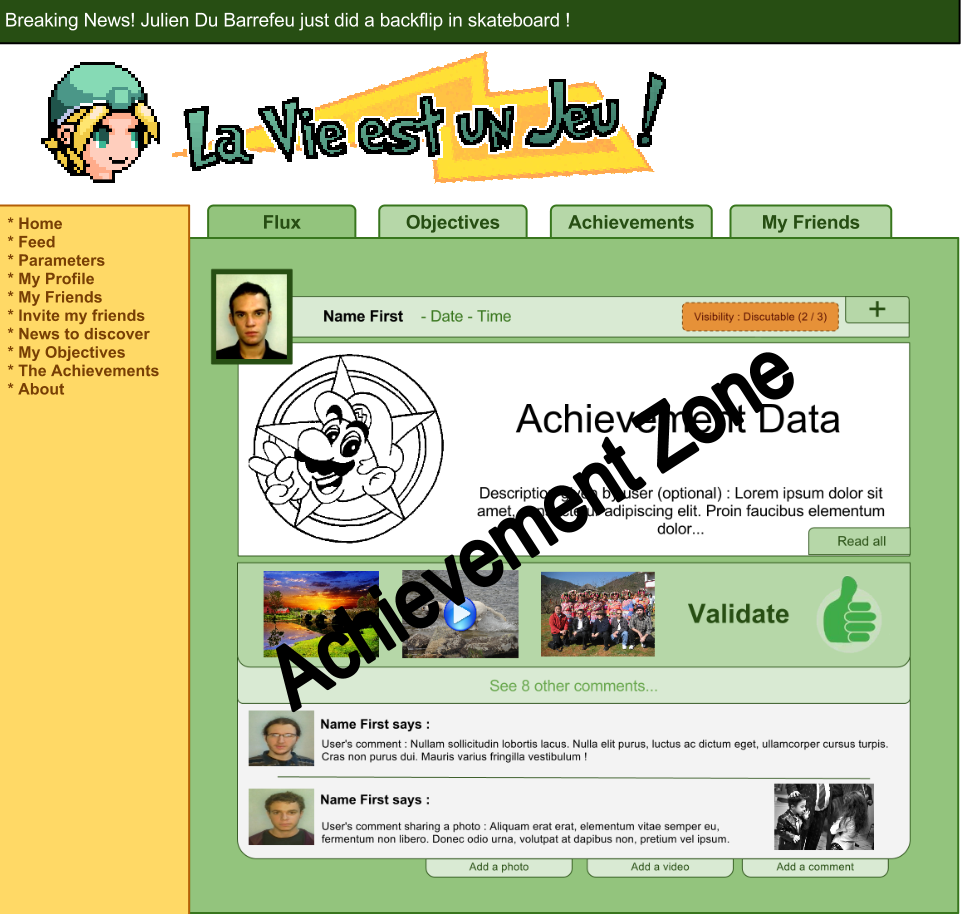
\includegraphics [width = 15cm]{img/accueil.png}
  \end{center}
\end{figure}


\subsection{Flow tab}

The Flow tab will be located in the middle of the main page and will feature displays the most recent "Achievements" made by the social network and to validate the circle of friends.\\

This feed will contain all the actions of contacts:

\begin{itemize}
  \item "Achievements" to validate (see details below);
  \item the goals they set for themselves;
  \item new contacts;
  \item new on the site (or new information "Achievements").
\end{itemize}

\newpage

\subsection{Details of an "achievement"}

Each "achievement" will have a validation function to the image of ``buttons'' I like Facebook or ``+1' 'Google +. It will allow users to indicate that they validate the publication in question. The validation support like the comments may be simple formatted text, picture and / or video. The photo (or "avatar") of the user will appear and the description of "achievement", next to it. It will also be possible to post comments below evidence of validation. A tab "More" will take place every "achievement" to get more information.\\

\begin{figure} [H]
  \begin{center}
    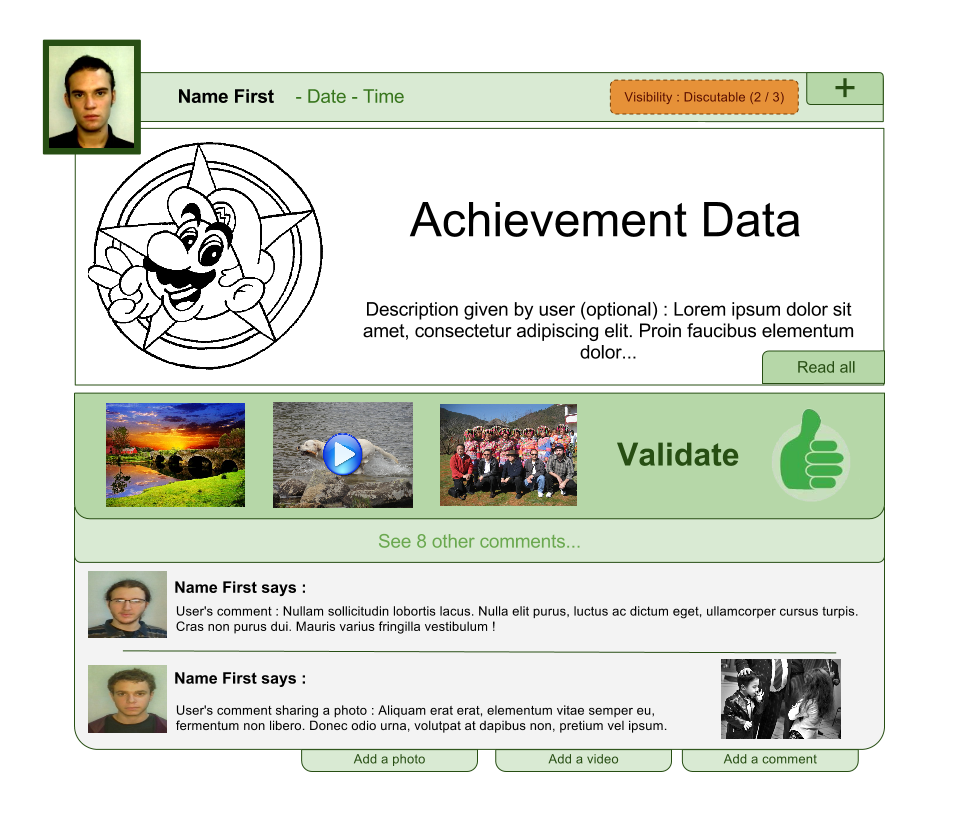
\includegraphics [width = 15cm]{img/achievement.png}
  \end{center}
\end{figure}

\subsection{Achievements tab}

The user can select packages that contain the "Achievements" to accomplish. The packs will be available all classified by theme and in a subcategory, but the platform will first the user packs of "Achievements" corresponding to the interests of the latter, or its bracket Age. Once a package is selected, the user can also define some "Achievements" as its objectives, and so notify its network.

\subsection{Objectives tab}

The Objectives tab allows the user to build a list of daily goals or things to do before dying completely. The purpose is to filter the "Achievements" that the user does not wish to make an immediate and so clear that they will accomplish in the short term. The page is intended to be regularly consulted: it is from this tab the user can announce the end of a goal, and thus obtain an "achievement" if his friends confirm the validation of the latter.

\subsection{Contacts tab}

The user can see here their contact list and profiles of these, but also group contacts by group. User groups can then assign degrees of sensitivity.\\
The sensitivity ranges from 0 to 3 and to share the "Achievements" to contacts of their choice. See below.

\subsection{Profile Page}

The Profile page contains information and allows a user to modify them. If the user is viewing the profile page of another member, he has the opportunity to interact with it in different ways (sending a message, request to add in the circle of friends, ...).\\
The profile page contains mainly badges "achievement" as a hunting scene. The user can click on the "achievement" for the full (text, photos, videos, comments).

\section{Application} Smartphone

As for smartphones, we decided to use the internet to develop an interface based on the technology we use for our website, namely Ocsigen. This will allow us to be consistent in our guideline of code. This interface will be charged on all smartphone platforms. The advantage of this method lies in its total portability and is a continuation of the challenge we set ourselves: to use functional programming for our project.

\section{API}

The API would provide developers access to the essential features of the site. We can come back, for a given user, and according to the wishes of the latter (token of acceptance), the list of "Achievements".


%% ------------------------------------------------ % ---------------------%

\chapter{A Technology brand new, original and effective}

\section{Ocsigen, web server and powerful framework in OCaml}

The technology used is called ``Ocsigen'' is a web server and a powerful framework entirely in OCaml.\\
  \\
Functional programming is completely adapted to the field of web as described in numerous articles on the internet, like this: \\
\url{http://www-lipn.univ-paris13.fr/~loddo/funding/projet-hyper-learning.pdf} \\
\\
Its strong typing solves many security problems that may be encountered in PHP for example.\\

\begin{figure} [H]
  \begin{center}
    
\includegraphics [width = 13cm]{img/ocsigen.png}
  \end{center}
\end{figure}

The framework is particularly well done and offers several levels of such session: Tabbed sessions, sessions by traditional client sessions per user (connected with the same login in several places), sessions with user groups and sessions "persistent" (retained after logging out).\\

\newpage

Because it is recent, it was conceived and designed for HTML5, Javascript and the latest client-side web technologies. When programming with Ocsigen, we realize a truly comprehensive program compiled and run. The language used is the same: OCaml for the client side as the server side.\\
\\
OCaml for easy handling of a tree, the generated code in HTML is done from an AST necessarily valid.\\
\\
To learn more about this little gem: \\
\url{http://ocsigen.org/}

\section{OCaml binding but ensuring stability and security}

The advantages and contraites of functional programming is also applicable in programming with Ocsigen.\\
\\
When you begin to write a program, even if the have started with a good foundation, it usually ends with a gas plant. And when you change something in one place, another feature to another place that depended on it becomes non-functional, and it takes time before one realizes it, often in production.\\

\begin{figure} [H]
  \begin{center}
    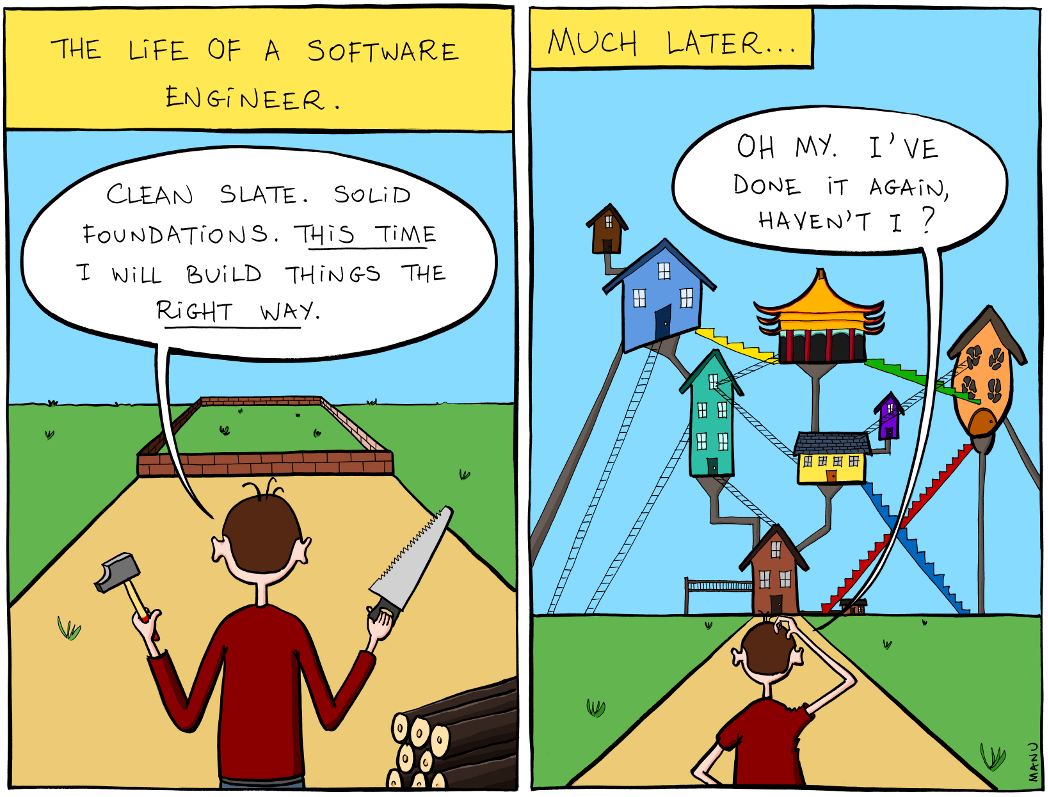
\includegraphics [width = 13cm]{img/proj.png}
  \end{center}
\end{figure}

\newpage

With OCaml and Ocsigen, a compiler is used very strict and strong typing. No deviation is tolerated!\\
Thus, if we modify a part of the program and it has an effect on another feature, then the program simply does not compile until everything is wrong.\\

This is very limiting for developers wishing to quickly create small applications without taking the head as they spend more time to ensure that the program compiles to realize the functionality itself.\\
For us, it's ideal. We know that by choosing this technology, we will spend much more time to design and build our project if we had chosen another more conventional technology for the web. But our ambitions are big on this project and we want to ensure its security, stability, performance, its purity and its total absence of bugs. We know that this solution corresponds exactly to our expectations.
\\

\section{Portability client / server}

\subsection{Server}

Ocsigen is a very new technology. The development of various services
started many years ago but the pooling of each output and
for final production use as of March 2012 with the release
version 2.0.\\
\\
Therefore, the server Ocsigen and all its associated modules not working
for now only on very few distributions. It fontionne on some
distrubutions Linux known as Ubuntu, Debian or Arch Linux. To date 
it does not work on Microsoft Windows, Apple Mac OS X or the 
BSD distributions. \\
\\
We still decided to highlight innovation over
the portability of our project. Our server is not portable.

\subsection{Client}

To overcome this disadvantage binding, we decided to make our
Ultra portable client-side service.\\
\\
The choice of using client-side Ocsigen évidante since this is 
technology is adapted to three use cases that represent access
\textit{via} a landline, smartphone or tablet. Under
the mobile web version Ocsigen manages over many features 
specific to mobile devices:
\begin{itemize}
  \item Tactile (touch simple, touching slipped, ...)
  \item Geolocation
  \item Orientation
  \item Camera
  items:
\end{itemize}

\begin{figure} [H]
  \begin{center}
    
\includegraphics [width = 8cm]{img/browsers.png}
  \end{center}
\end{figure}

Our service is guaranteed to be usable on three different platforms:

\begin{itemize}
  \item standard Web browsers
    \begin{itemize}
      \item Chrome
      \item Mozilla Firefox
      \item Internet Explorer
      \item Apple Safari
      \item Opera
    \end{itemize}
  \item Terminals mobile phone format
    \begin{itemize}
      \item Android
      \item iOS
      \item Windows Mobile
      \item BlackBerry
    \end{itemize}
  \item Shelves
    \begin{itemize}
      \item iPad
      \item Android Tablet
    \end{itemize}
\end{itemize}

\begin{figure} [H]
  \begin{center}
    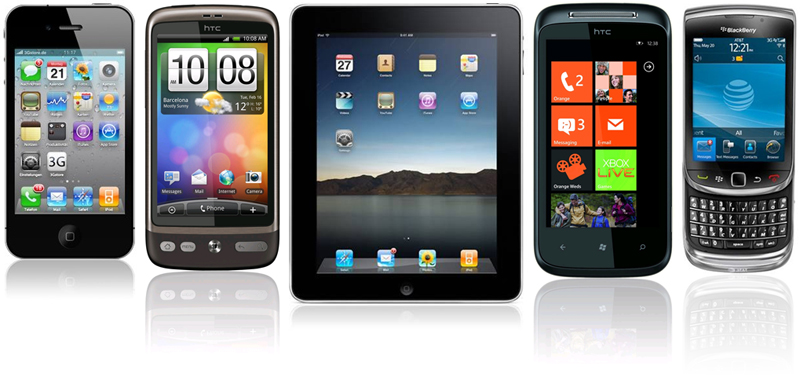
\includegraphics [width = 13cm]{img/mobiles.jpg}
  \end{center}
\end{figure}

For Any of these three platforms, we will have a different interface
and adapted to the resolution and functionality.\\
For each type of device, we will have a different program,
coded in the language appropriate to it, using our service Ocsigen
\textit{via} API developers detail later.\\
In all, we will:
\begin{itemize}
  \item three different services Ocsigen
  \item 6 different mobile applications, in their respective languages
\end{itemize}

We can therefore say that ``La Vie Est Un Jeu'' is \textbf{ultra-portable}.

%% ------------------------------------------------ % ---------------------%

\chapter{Description of the database}

\section{Description of the first level of tests}

\begin{itemize}
  \item Create an Account
  \item Access restriction by circles
  \item listing of "Achievements" already in the database
  \item Selection of "Achievements" from those available.
  \item Weighting "Achievements".
  \item classification: tests of different scoring algorithms.
  \item Restriction of the achievements for a class of users (those at level 3 will not be available at least 18 years of age and those at Level 2 under 14).
\end{itemize}

\section{Outline of the database}

\begin{figure} [H]
  \begin{center}
    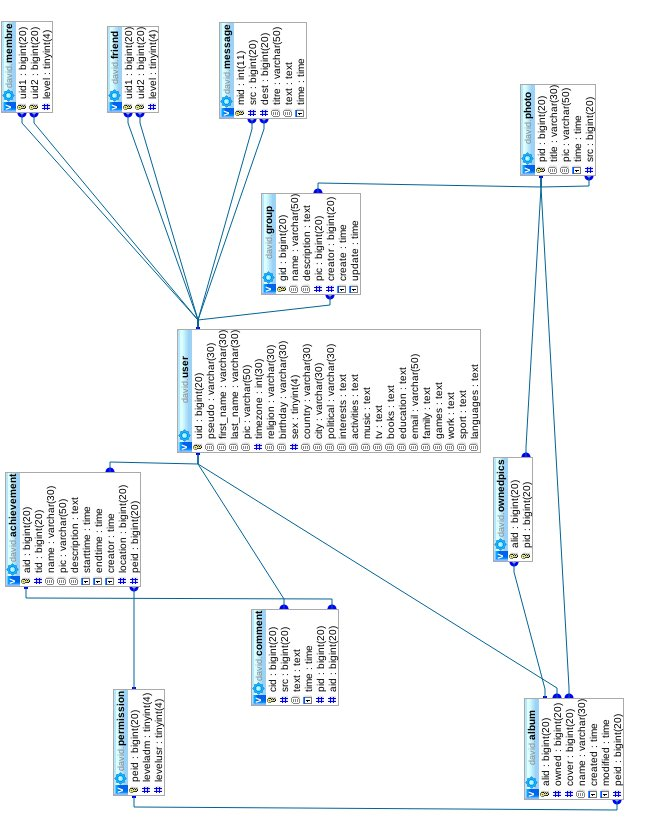
\includegraphics [width = 18cm]{img/imgdb.jpg}
  \end{center}
\end{figure}

\section{Technology and portability of the database}

For the database we use a service that we have imposed
\textbf{Ocsigen}, the technology we use for our entire project.\\
This service is called \textbf{Macaque}. It offers a functional approach
and strongly typed management database.\\
This service is based on PostgreSQL and it is possible to interact with the
database with other systems using PostgreSQL.
However, the interaction with the database since our Ocsigen
can be done with macaque.\\
\\
To use other types of data bases when needed
for the future, we plan to offer converters database.\\
We propose a PostgreSQL to MySQL converter in another language and
the need for other converters.

\begin{figure} [H]
  \begin{center}
    
\includegraphics[width = 13cm]{img/macaque.png}
  \end{center}
\end{figure}

%% ------------------------------------------------ % ---------------------%

\chapter{physical and human environment of the project}

\section{Hardware Environment}

Our project runs on a server Ocsigen. It is installed on a Dell PRO Dedibox funded by project members.

\vspace{20pt}

\begin{tabular}{| c | c |}
  \hline
   Dell PowerEdge ® Server & R210 \\
  \hline
  Processor & 1x Intel ® Xeon ® L3426 \\
  \hline
  Architecture & 4x 1.86GHz, 64-Bit, Virtualization \\
  \hline
  RAM & 16 GB DDR3 ECC \\
  \hline
  HDD & 2 x 2TB SATA2 Raid 0 / Raid 1 HARD (H200) \\
  \hline
  Monthly price 49.99 euros HT & \\
  \hline
\end{tabular}

\vspace{20pt}

\section{Costs}

\begin{itemize}
  \item A developer account for each store application (IOS: AppStore (99 \$), Play Google (Android: 25 \$) and Windows Phone Marketplace (99 \$)) for mobile applications.
  \item A dedicated server, initially built for the development of the site can handle only a few users connected simultaneously at about 60 euros per month.
  \item A production server, which will later be used up to 600 euros per month.
  \item We see later, once the application is fully completed, to hire a graphic designer for "Achievements".
\end{itemize}

\section{Environment} and implementation tools

To communicate and discuss the project, our working group relies on several tools.

\begin{itemize}
  \item The project has its official IRC channel (\#life-eip on irc.epitech.net), whose goal is to provide quick support to users and contributors by managing a chat history.
  \item Additionally, the project team has access to a mailing list (hosted by google groups).
  \item It manages all documents relating to the project's progress through google documents.
  \item Documentation can be found on the showcase site: \url{http://eip.epitech.eu/2014/lavieestunjeu/}
  \item We have a bug tracker, wiki and tickets to a private GitHub repository.
\end{itemize}

\section{Technical Architecture}

\begin{itemize}
  \item The project is based on a Web environment in OCaml, so the main component is the web server
        \href{http://ocsigen.org/}{Ocsigen}.
  \item The project will also build on \href{http://ocsigen.org/js_of_ocaml/}{js\_of\_ocaml}, a tool for compiling OCaml JavaScript.
  \item It will manage a database using \href{http://ocsigen.org/macaque/}{Macaque}, another project initiated by INRIA.
\end{itemize}

For details, see the chapter on the technologies used.

\section{Users Information Security}

\begin{itemize}
  \item Implementation of a solution of "privacy level", a user can define a level of privacy for each user on its network. 

\begin{figure} [H]
  \begin{center}
    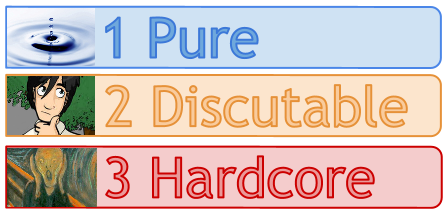
\includegraphics [width = 10cm]{img/confidentialite.png}
  \end{center}
\end{figure}

\end{itemize}

\section{Sensitive points}

\begin{itemize}
  \item Information security is a priority for us. We will therefore pay close attention to what users are always aware at any time who has access to what information.
  \item We want to keep our ideas secret until we have a basic version available.
  \item The stability and security is our priority and will be provided through the use of Ocsigen.
\end{itemize}

%% ------------------------------------------------ % ---------------------%

\chapter{Project Organization}

\section{Planning}

From a global perspective, the project will proceed in three main sections: documentation, development and production.\\

\subsection{First year: Documentation, Design}

Before turning to the concrete realization of the product, we will devote ourselves to the drafting of several key documents to the project runs smoothly. Indeed, it is necessary to precisely define the details of the project, design, explore the various tools and technologies at our disposal and make choices, or develop partnerships.\\
Among the documents produced are:

\begin{itemize}
  \item 50 words
  \item Study of the existing
  \item A detailed study
  \item Terms of Reference (3 versions)
  \item Gantt Chart
  \item Review Architecture
\end{itemize}

We will continue this study until September 2012.\\

\newpage

\subsection{Second year: Development, Code, Tests}
Once the tools at hand, the specific and defined roles, we will begin to develop the product.\\
\begin{itemize}
  \item Hello World! (01/08/12)
  \item \textbf{Connection}: (08/01/12)
  \item Form website (01/08/12)
  \item Facebook / Google + (01/08/12)
  \item Home (01/08/12)
  \item \textbf{BDD Management}: (01/08/12)
  \item Deployment database (01/08/12)
  \item categories and subcategories of Achievements (08/29/12)
  \item Course categories (29/08/12)
  \item simple Achievements (29/08/12)
  \item Contact Management (01/10/12)
  \item Contacts Facebook / Google + (10/01/12)
  \item Set up security and sharing (01/10/12)
  \item Share Facebook / Google + (01/11/12)
  \item Create Flow (01/11/12)
  \item \textbf{Management Achievements}: (01/11/12)
  \item Custom text (01/12/12)
  \item Videos and photos (01/11/12)
  \item Simple Comments (01/01/13)
  \item Comments videos and photos (01/01/13)
  \item User Profile page (01/01/13)
  \item Objectives Achievements by users (01/02/13)
  \item Filtering to display RSS (01/01/13)
  \item Finalization users (avatars, info ...) (01/02/13)
  \item Completing Achievements (01/03/13)
  \item guide discovery site (04/01/13)
  \item Finalization Site / Testing phase (01/04/13)
  \item Output of a first version of the site (06/01/13)
\end{itemize}

Late in the second year after the completion of the project, we will devote at least one month prior to testing to production. These tests would be \\
We believe putting it into production for a final version in September 2013.\\

\newpage

\subsection{Third year: Release, partennariats commercial, business creation}

The last period will be devoted to communication issues, and to a lesser degree of development. Thus, during the last year of the project, we will try to express it in various ways to create community essential to our platform, in addition to the finalization of the technical product. We can thus benefit from user feedback in order to correct anomalies and refine the platform.\\
We wish to obtain partennariats to advertise our business platform.\\
We wish to register our project in many contests of innovation and startups to gain visibility and audience, and why not additional funding.\\
\\
In short, the third year is dedicated to making this project a \textbf{success}.

\begin{figure} [H]
  \begin{center}
    
\includegraphics [width = 12cm]{img/corporate.jpg}
  \end{center}
\end{figure}

\newpage

\section{The Team}

During the product development team will be dispersed in several countries, making any teamwork difficult. We will allocate tasks so as to be able to work relatively autonomously: our project is composed of several distinct elements, we will arrange to not share one between members located in different places.\\

\subsection{Distribution of roles}

Below is the list of officers assigned to each category of tasks
Project\\
Officials are not necessarily those that will perform the tasks, but
are the ones who have the responsibility to ensure that these are
made, making them themselves or by distributing the work.

\subsection{Documentation, Design}

\begin{itemize}
  \item \textbf{Guillaume Caradec} handles the overall management of project
  \item \textbf{Barbara Lepage} directs the technical part.
  \item \textbf{Barbara Lepage} is responsible of the showcase site
  \item \textbf{Barbara Lepage} is responsible for documentation
  \item \textbf{Lassagne David} is responsible for design
  \item \textbf{Barbara Lepage} is responsible for training and OCaml Ocsigen
  \item \textbf{Nicolas Klarman} is grand master of "Achievements"
\end{itemize}

\subsection{Development, code, tests}

\begin{itemize}
  \item \textbf{Barbara Lepage} is responsible for application development side
    Server.
  \item \textbf{Louvigny Guillaume} is responsible for development
    client-side applications for the web interface
  \item \textbf{Guillaume Caradec} takes care of the ergonomics, interface, the
    overall design
  \item \textbf{Lassagne David} is responsible for database architecture
  \item \textbf{Guillaume Louvigny} is responsible SQL
  \item \textbf{Le-Cor Wilfried} is responsible of the Android development
  \item \textbf{Francois Glorieux} is responsible of the Windows development
  \item \textbf{Youssef El-Outmani} is responsible for developing Blackberry
  \item \textbf{Nicolas Klarman} is responsible for developing iOS
  \item \textbf{Frank Lenormand} is responsible for multimedia (photos, videos, ...)
  \item \textbf{Guillaume Louvigny} is responsible social networks (Facebook,
    + Google, Twitter, ...)
  \item \textbf{Frank Lenormand} is responsible commit
  \item \textbf{Corsin Simon} is responsible for third party developers (API)
  \item \textbf{Wilfried Le Cor} User interaction is responsible
  \item \textbf{Nicolas Klarman} is responsible Gameplay
  \item \textbf{Francois Glorieux} community aspect is responsible
  \item \textbf{Corsin Simon} is responsible for testing the Release
\end{itemize}

\subsection{Communication, company}

\begin{itemize}
  \item \textbf{Guillaume Caradec} is responsible communication
  \item \textbf{Guillaume Caradec} is sales manager
  \item \textbf{Barbara Lepage} is responsible for business
  \item \textbf{Barbara Lepage} is responsible for innovation
  \item \textbf{Barbara Lepage} is responsible for funding
\end{itemize}

\subsection{Tools}

We have at our disposal various tools to get organized and communicate more easily: \\

\begin{itemize}
  \item a mailing list and an IRC channel, to treat all the various issues;
  \item a Google Docs file, so you can share documents related to the project and writing;
  \item Gtalk, Google's application for organizing video conferences via a browser;
  \item a Git;
  \item using Doodle to schedule meetings more easily.
\end{itemize}

Group members will meet \textbf{weekly} to discuss project progress, and unanticipated set of short-term goals.


\section{Detailed schedule with specific dates}

Please see the attached file \texttt{2014\_GAN3\_EN\_lavieestunjeu.pdf}. It contains the Gantt chart of our project.

%% ------------------------------------------------ % ---------------------%

\chapter{Conclusion}

\section{Document conclusion}

This paper presented the specification so our EIP, ``La Vie Est Un Jeu'' \\
\\
We have described all the features that will be proposed, which includes both the website and mobile applications.\\
\\
Was also presented the definition of the database on all applicable platforms covered.\\
\\
The API destined for third-party developers had also been defined.\\
\\
Finally, he detailed also those who can win the project, and estimated the various constraints imposed by it be they financial or organizational.\\

\section{SWOT}

\begin{figure} [H]
  \begin{center}
    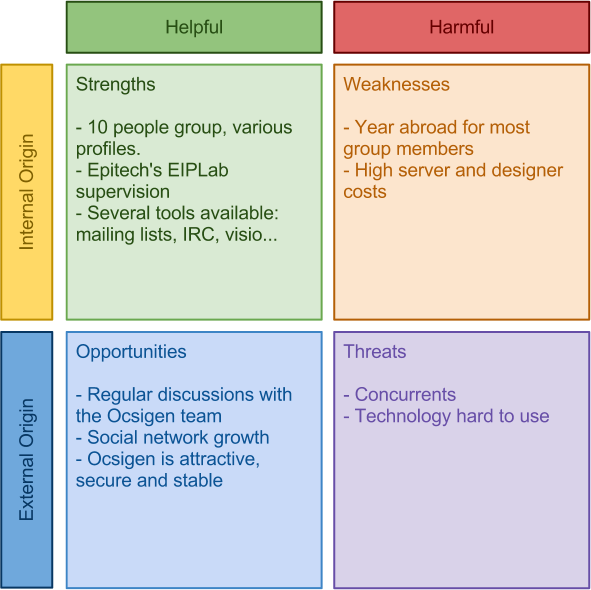
\includegraphics [width = 14cm]{img/swot_en.png}
  \end{center}
\end{figure}

%% ------------------------------------------------ % ---------------------%

\chapter{Appendix}

\section{Location of team members during the second year of the project}

\begin{tabular}{| c | c |}
  \hline
  Lepage Barbara and Long Beach & Berkey, USA \\
  \hline
  Caradec Guillaume & Paris, France \\
  \hline
  Corsin Simon & Paris, France \\
  \hline
  Francois Glorieux & Peking University, China \\
  \hline
  Klarman & Nicolas Paris, France \\
  \hline
  Lassagne David & Peking University, China \\
  \hline
  Louvigny Guillaume & Paris, France \\
  \hline
  El-Youssef Outmani & Peking University, China \\
  \hline
  The Cor-Wilfried & Sweden \\
  \hline
  Frank & Lenormand Finland \\
  \hline
\end{tabular}

\newpage

\section{Glossary}


\begin{description}
\item [Algorithm]
And finite sequence of unambiguous instructions to give the answer to a problem.
\item [API]
In ``French'' Programming Interface, is an interface provided by a computer program for the interaction of programs with each other.

\item [mobile application]
A mobile application is an application developed to be installed on mobile electronic devices.

\item [Web Architecture]
Web-based architecture means the general structure inherent in a web environment.

\item [Database]
A database is a lot of information stored in a computing device.

\item [Breaking news]
Latest News in French ``''.

\item [Bug Tracker]
In French ``Software'' issue tracking, software to help users and developers to improve software quality by finding the flaws of such software.

\item [Specifications]
Specification is to simply define the specifications of a product or service to achieve.

\item [Filing]
A repository is a centralized storage and organizing data.

\item [Gantt]
A Gantt chart is a tool used in scheduling and project management and for viewing in time the various tasks a project component.

\item [Slideshow]
A slideshow is a sequence of images or documents connected by and effects on which it is possible to sound.

\item [Doodle]
Doodle.com is a website planning and survey of the Swiss company Doodle AG.

\item [GitHub]
Github is a Web service hosting and management of software development, Git using the program. 

\item [Google Docs]
Google Docs is a result of changes in Google Spreadsheets, word processing software. These programs allow a merged online collaboration.

\item [Google Talk]
Google Talk is proprietary software and instant messaging service and VoIP Jabber-based and developed by Google.

\item [IRC]
IRC is a protocol text communication on the internet.

\item [JavaScript]
JavaScript is a scripting programming language used primarily for interactive web pages.

\item [Login]
``ID'' in French, information enabling a person to identify themselves to a system.

\item [Mailing list]
In French ``mailing list'', specific use of electronic mail that allows direct mail information to users who are enrolled.

\item [into production]
Provision ``total'' of a service or product.

\item [Ocaml]
Formerly known as Objective Caml is the most advanced implementation of Caml programming language.

\item [Ocsigen]
Web development framework, developed by the French laboratory PPS.

\item [Network]
Mesh of links between different computer equipment allowing sharing of information.

\item [social network]
Set of social identities, such as individuals or organizations linked together by bonds created during social interactions.

\item [Service]
Adds value to a product or work required to ensure a company or an individual.

\item [storefront]
Website composed of a few pages with a company. Allows a company to communicate with the world.

\item [Smartphone]
With mobile phone also features a PDA. It provides basic functionality such as calendar, calendar, web browsing, consulting e-mail, instant messaging, GPS ...

\item [Android]
Operating system using the Linux kernel for smartphones, mobile PDAet designed by Android, a startup acquired by Google.

\item [IOS]
Mobile operating system developed by Apple for iPhone, iPod touch, and the iPad. It is derived from Mac OS X with which it shares foundations.

\item [Windows Phone]
Mobile operating system developed by Microsoft as the successor to Windows Mobile, its previous software platform.

\item [Beta]
Test version includes all the features of a program. It is through this version that testers back any problems.

\item [Wiki]
Collaborative space where users are invited to write papers.


\end{description}
\end{document}
